20. $y=\cfrac{x^2-6x+5}{x-|x-2|}=\begin{cases}\cfrac{(x-5)(x-1)}{2},\ x\geqslant2,\\ \cfrac{(x-5)(x-1)}{2x-2},\ x<2,\ x\neq1.\end{cases}=
\begin{cases}\cfrac{1}{2}x^2-3x+\cfrac{5}{2},\ x\geqslant2,\\ \cfrac{x-5}{2},\ x<2,\ x\neq1.\end{cases}$
$$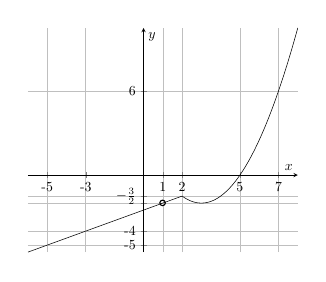
\begin{tikzpicture}[scale=0.5]
\begin{axis}[
    axis lines = middle,
    grid=major,
    legend pos={south west},
    xlabel = {$x$},
    %xlabel style={below right},
    ylabel = {$y$},
    xtick={-5, -3,1, 2,5,7},
    xticklabels={-5, -3,1, 2,5,7},
    ytick={-5,-4,-2,-1.5,6},
    yticklabels={-5,-4,$ $,$-\frac{3}{2}$,6},
                  ]
	\addplot[domain=-6:2, samples=100, color=black] {(x-5)/(2)};
    \addplot[domain=2:8, samples=100, color=black] {(x*x-6*x+5)/2};
	%\addlegendentry{$\text{Рис. 1}$};
\end{axis}
\draw (3.42,1.25) circle (2pt);
%\draw (3.7,3.05) circle (2pt);
\end{tikzpicture}$$
